% Compatibility shims for the local hyperref/LaTeX combination.
\providecommand\IfDocumentMetadataT[1]{}
\providecommand\IfDocumentMetadataTF[2]{#2}
\documentclass[aspectratio=169,9pt]{beamer}
\NeedsTeXFormat{LaTeX2e}
\RequirePackage{fontspec}
\RequirePackage{amsmath,amssymb,mathtools}
\RequirePackage{booktabs}
\RequirePackage{graphicx}
\RequirePackage{microtype}
\RequirePackage{ragged2e}
\RequirePackage{hyperref}
\RequirePackage{tikz}
\usetikzlibrary{arrows.meta,positioning,calc}

\IfFontExistsTF{Avenir Next}{\setsansfont{Avenir Next}}{\setsansfont{TeX Gyre Heros}}

\definecolor{QXNavy}{HTML}{0C2852}
\definecolor{QXRed}{HTML}{982A34}
\definecolor{QXGraphite}{HTML}{20242A}
\definecolor{QXMuted}{HTML}{5B6470}
\definecolor{QXRedTitle}{HTML}{F4E8EA}
\definecolor{QXRedBody}{HTML}{F9F5F5}
\definecolor{QXBlueTitle}{HTML}{EBEEF1}
\definecolor{QXBlueBody}{HTML}{F5F6F8}
\definecolor{QXGreen}{HTML}{3B5526}
\definecolor{QXDivider}{HTML}{D9DEE4}

\usetheme{default}
\usefonttheme{professionalfonts}
\setbeamertemplate{navigation symbols}{}
\setbeamersize{text margin left=0.54cm,text margin right=0.54cm}
\setbeamercolor{background canvas}{bg=white}
\setbeamercolor{normal text}{fg=QXGraphite,bg=white}
\setbeamercolor{frametitle}{fg=white,bg=QXNavy}
\setbeamercolor{structure}{fg=QXNavy}
\setbeamercolor{alerted text}{fg=QXRed}
\setbeamercolor{qx red title}{fg=QXRed,bg=QXRedTitle}
\setbeamercolor{qx red body}{fg=QXGraphite,bg=QXRedBody}
\setbeamercolor{qx blue title}{fg=QXNavy,bg=QXBlueTitle}
\setbeamercolor{qx blue body}{fg=QXGraphite,bg=QXBlueBody}
\setbeamercolor{qx accent line}{bg=QXRed}
\setbeamercolor{qx divider line}{bg=QXDivider}
\setbeamercolor{qx foot}{fg=QXMuted,bg=white}
\setbeamercolor{qx takeaway}{fg=white,bg=QXNavy}
\setbeamercolor{qx placeholder}{fg=QXMuted,bg=QXBlueBody}
\setbeamerfont{frametitle}{size=\large,series=\bfseries}
\setbeamerfont{block title}{size=\normalsize,series=\bfseries}
\setbeamerfont{footline}{size=\scriptsize}
\providecommand{\qxdecklabel}{Quispe \& Xu (2026) · language-frontier audit}

\setbeamertemplate{frametitle}{%
  \nointerlineskip
  \begin{beamercolorbox}[wd=\paperwidth,ht=0.62cm,dp=0.23cm,leftskip=0.48cm]{frametitle}%
    \usebeamerfont{frametitle}\insertframetitle
  \end{beamercolorbox}%
  \nointerlineskip
  \hbox{%
    \begin{beamercolorbox}[wd=1.05cm,ht=0.018cm,dp=0cm]{qx accent line}\end{beamercolorbox}%
    \begin{beamercolorbox}[wd=\dimexpr\paperwidth-1.05cm\relax,ht=0.018cm,dp=0cm]{qx divider line}\end{beamercolorbox}%
  }%
}

\setbeamertemplate{footline}{%
  \leavevmode\hbox{%
    \begin{beamercolorbox}[wd=.83\paperwidth,ht=0.26cm,dp=0.10cm,leftskip=.52cm]{qx foot}%
      \qxdecklabel
    \end{beamercolorbox}%
    \begin{beamercolorbox}[wd=.17\paperwidth,ht=0.26cm,dp=0.10cm,rightskip=.52cm plus1fil]{qx foot}%
      \insertframenumber/\inserttotalframenumber
    \end{beamercolorbox}%
  }%
}

\newcommand{\E}{\mathbb{E}}
\newcommand{\ATT}{\operatorname{ATT}}
\newcommand{\qxredblock}[2]{%
  \begin{beamercolorbox}[wd=\linewidth,sep=0.10cm,leftskip=0.07cm,rightskip=0.07cm]{qx red title}\usebeamerfont{block title}#1\end{beamercolorbox}%
  \nointerlineskip
  \begin{beamercolorbox}[wd=\linewidth,sep=0.13cm,leftskip=0.10cm,rightskip=0.10cm]{qx red body}#2\end{beamercolorbox}%
}
\newcommand{\qxblueblock}[2]{%
  \begin{beamercolorbox}[wd=\linewidth,sep=0.10cm,leftskip=0.07cm,rightskip=0.07cm]{qx blue title}\usebeamerfont{block title}#1\end{beamercolorbox}%
  \nointerlineskip
  \begin{beamercolorbox}[wd=\linewidth,sep=0.13cm,leftskip=0.10cm,rightskip=0.10cm]{qx blue body}#2\end{beamercolorbox}%
}
\newcommand{\qxtwocol}[4]{%
  \noindent\hspace*{0.12cm}%
  \begin{minipage}[t]{#1\linewidth}\vspace{0pt}#2\end{minipage}%
  \hfill
  \begin{minipage}[t]{#3\linewidth}\vspace{0pt}#4\end{minipage}%
  \hspace*{0.12cm}\par
}
\newcommand{\qxtakeaway}[1]{%
  \begin{beamercolorbox}[wd=\linewidth,sep=0.12cm,leftskip=0.10cm,rightskip=0.10cm]{qx takeaway}
    \small\bfseries #1
  \end{beamercolorbox}%
}


\begin{document}

% 1/5 — title
\begin{frame}[plain]
  \setbeamertemplate{footline}{}
  \vspace*{1.45cm}
  {\fontsize{19}{22}\selectfont\bfseries Agentic Delegation and the Language Frontier\par}
  \vspace{0.16cm}
  {\fontsize{12.5}{15}\selectfont What the threshold model predicts—and what the design cannot identify\par}
  \vspace{0.48cm}
  {\color{QXRed}\rule{\linewidth}{0.55pt}}
  \vspace{0.52cm}
  {\normalsize\bfseries Gabriel Saco\par}
  \vspace{0.06cm}
  {\normalsize August 29, 2026\par}
  \vspace{0.20cm}
  {\small Universidad del Pac\'ifico\par}
  \vspace{0.22cm}
  {\small\color{QXMuted}Quispe \& Xu (2026) · arXiv:2605.25438\par}
  \vspace{0.10cm}
  {\small\href{https://github.com/gsaco/ai-03-quispe/tree/branch1}{\color{QXNavy}\ttfamily github.com/gsaco/ai-03-quispe/tree/branch1}\par}
  \vfill
  {\scriptsize\color{QXMuted}AI Economic Modeling\hfill Five-minute paper audit\par}
\end{frame}

% 2/5 — paper and problem
\begin{frame}[t]{The paper and the developer's problem}
  \vspace{0.22cm}
  \qxredblock{Question and economic mechanism}{%
    \small
    \textbf{Question.} Does an agent expand the set of programming languages
    in which a developer can ship code? This is a \alert{production frontier},
    not a claim that the developer learns each language.

    \vspace{0.06cm}
    \textbf{Mechanism.} Conversational AI augments existing language skill;
    agentic AI adds delegated execution under human specification and verification.
  }

  \vspace{0.24cm}
  \qxblueblock{Choice problem for developer $i$, language $k$, month $t$}{%
    \small
    \qxtwocol{.53}{%
      Pre-agent menu $\mathcal M_1=\{S,C\}$; post-agent menu
      $\mathcal M_2=\{S,C,D\}$:
      \[
        m^*_{ikt}\in\arg\max_{m\in\mathcal M_g}V^m_{ikt},
        \qquad
        Z^g_{ikt}=\mathbb I(\max_mV^m_{ikt}\ge0).
      \]
      Monthly breadth is $N^g_{it}=\sum_k Z^g_{ikt}$.
    }{.39}{%
      \textbf{$S$:} own execution.\\[0.07cm]
      \textbf{$C$:} suggestion gain $\gamma s-r_C$.\\[0.07cm]
      \textbf{$D$:} agent execution $\lambda a z(A)$, net of verification
      $\kappa(a,s)$, compute $r_D$, and residual risk.
    }
  }
\end{frame}

% 3/5 — main result and conditions
\begin{frame}[t]{Main result: a conditional activation band}
  \setlength{\abovedisplayskip}{0.28em}
  \setlength{\belowdisplayskip}{0.28em}
  \vspace{0.12cm}
  \qxblueblock{Proposition 2 for an unfamiliar language}{%
    \small
    If conversational assistance has no value without a skill foothold,
    $\gamma\underline s-r_C\le0$, then $T^1=T^S$. If delegation lowers the
    threshold, $B\equiv T^S-T^D>0$, then
    \[
      Z^2-Z^1=\mathbb I(T^D\le\omega<T^S),
      \qquad
      \Pr(Z^2-Z^1=1)=F(T^S)-F(T^D).
    \]
  }

  \vspace{0.18cm}
  \qxredblock{Conditions that do the work}{%
    \small
    \qxtwocol{.46}{%
      \textbf{Theory}
      \begin{itemize}\itemsep0.04cm
        \item no conversational foothold in $k$;
        \item verification, compute, and residual-risk costs leave $B>0$;
        \item opportunity mass lies inside $[T^D,T^S)$;
        \item the developer can specify and verify.
      \end{itemize}
    }{.46}{%
      \textbf{Empirical interpretation}
      \begin{itemize}\itemsep0.04cm
        \item public, sustained adopters; “new” since Jan. 2024;
        \item not-yet adopters are valid counterfactuals;
        \item no time-varying project shock jointly moves adoption and languages.
      \end{itemize}
    }
  }

  \vspace{0.16cm}
  \qxtakeaway{Observed at adoption: +2.53 active languages and +1.19 newly used languages; these are event-time associations, not identified causal effects.}
\end{frame}

% 4/5 — what I did
\begin{frame}[t]{What I did: two pressure tests}
  \setlength{\abovedisplayskip}{0.24em}
  \setlength{\belowdisplayskip}{0.24em}
  \vspace{0.12cm}
  \qxredblock{1. The activation band does not uniquely require an agent}{%
    \small
    A generic productivity or fixed-cost improvement $\tau>0$ gives
    $T^G=T^1-\tau$ and therefore
    \[
      Z^G-Z^1=\mathbb I(T^1-\tau\le\omega<T^1).
    \]
    This is the same comparative static. Agent specificity comes from how the
    modes are assumed, not from the threshold result itself.
  }

  \vspace{0.18cm}
  \qxblueblock{2. A zero-effect selection counterexample}{%
    \small
    Let an unfamiliar-language project shock both trigger adoption and raise breadth:
    \[
      A_{it}=\mathbb I[P_{it}\ge c_i],\qquad
      Y_{it}=\mu_i+\lambda_t+\beta P_{it}+\tau A_{it}+\varepsilon_{it}.
    \]
    At first adoption,
    \[
      \widehat{\ATT}(e)=\tau+
      \beta\!\left[\E(P_{it}\mid G_i=g)-\E(P_{it}\mid G_i>t)\right].
    \]
    The repository simulation sets $\tau=0$ and still produces a sharp event-time jump.
  }

  \vspace{0.16cm}
  \qxtakeaway{The robustness checks clean the outcome; they do not exogenize the timing of adoption.}
\end{frame}

% 5/5 — hand check and verdict
\begin{frame}[t]{Hand check: where I did not believe the AI}
  \setlength{\abovedisplayskip}{0.22em}
  \setlength{\belowdisplayskip}{0.22em}

  \begin{columns}[T,onlytextwidth]
    \begin{column}{0.46\textwidth}
      \IfFileExists{hand/selection-derivation.jpg}{%
        \centering
        \fcolorbox{QXDivider}{white}{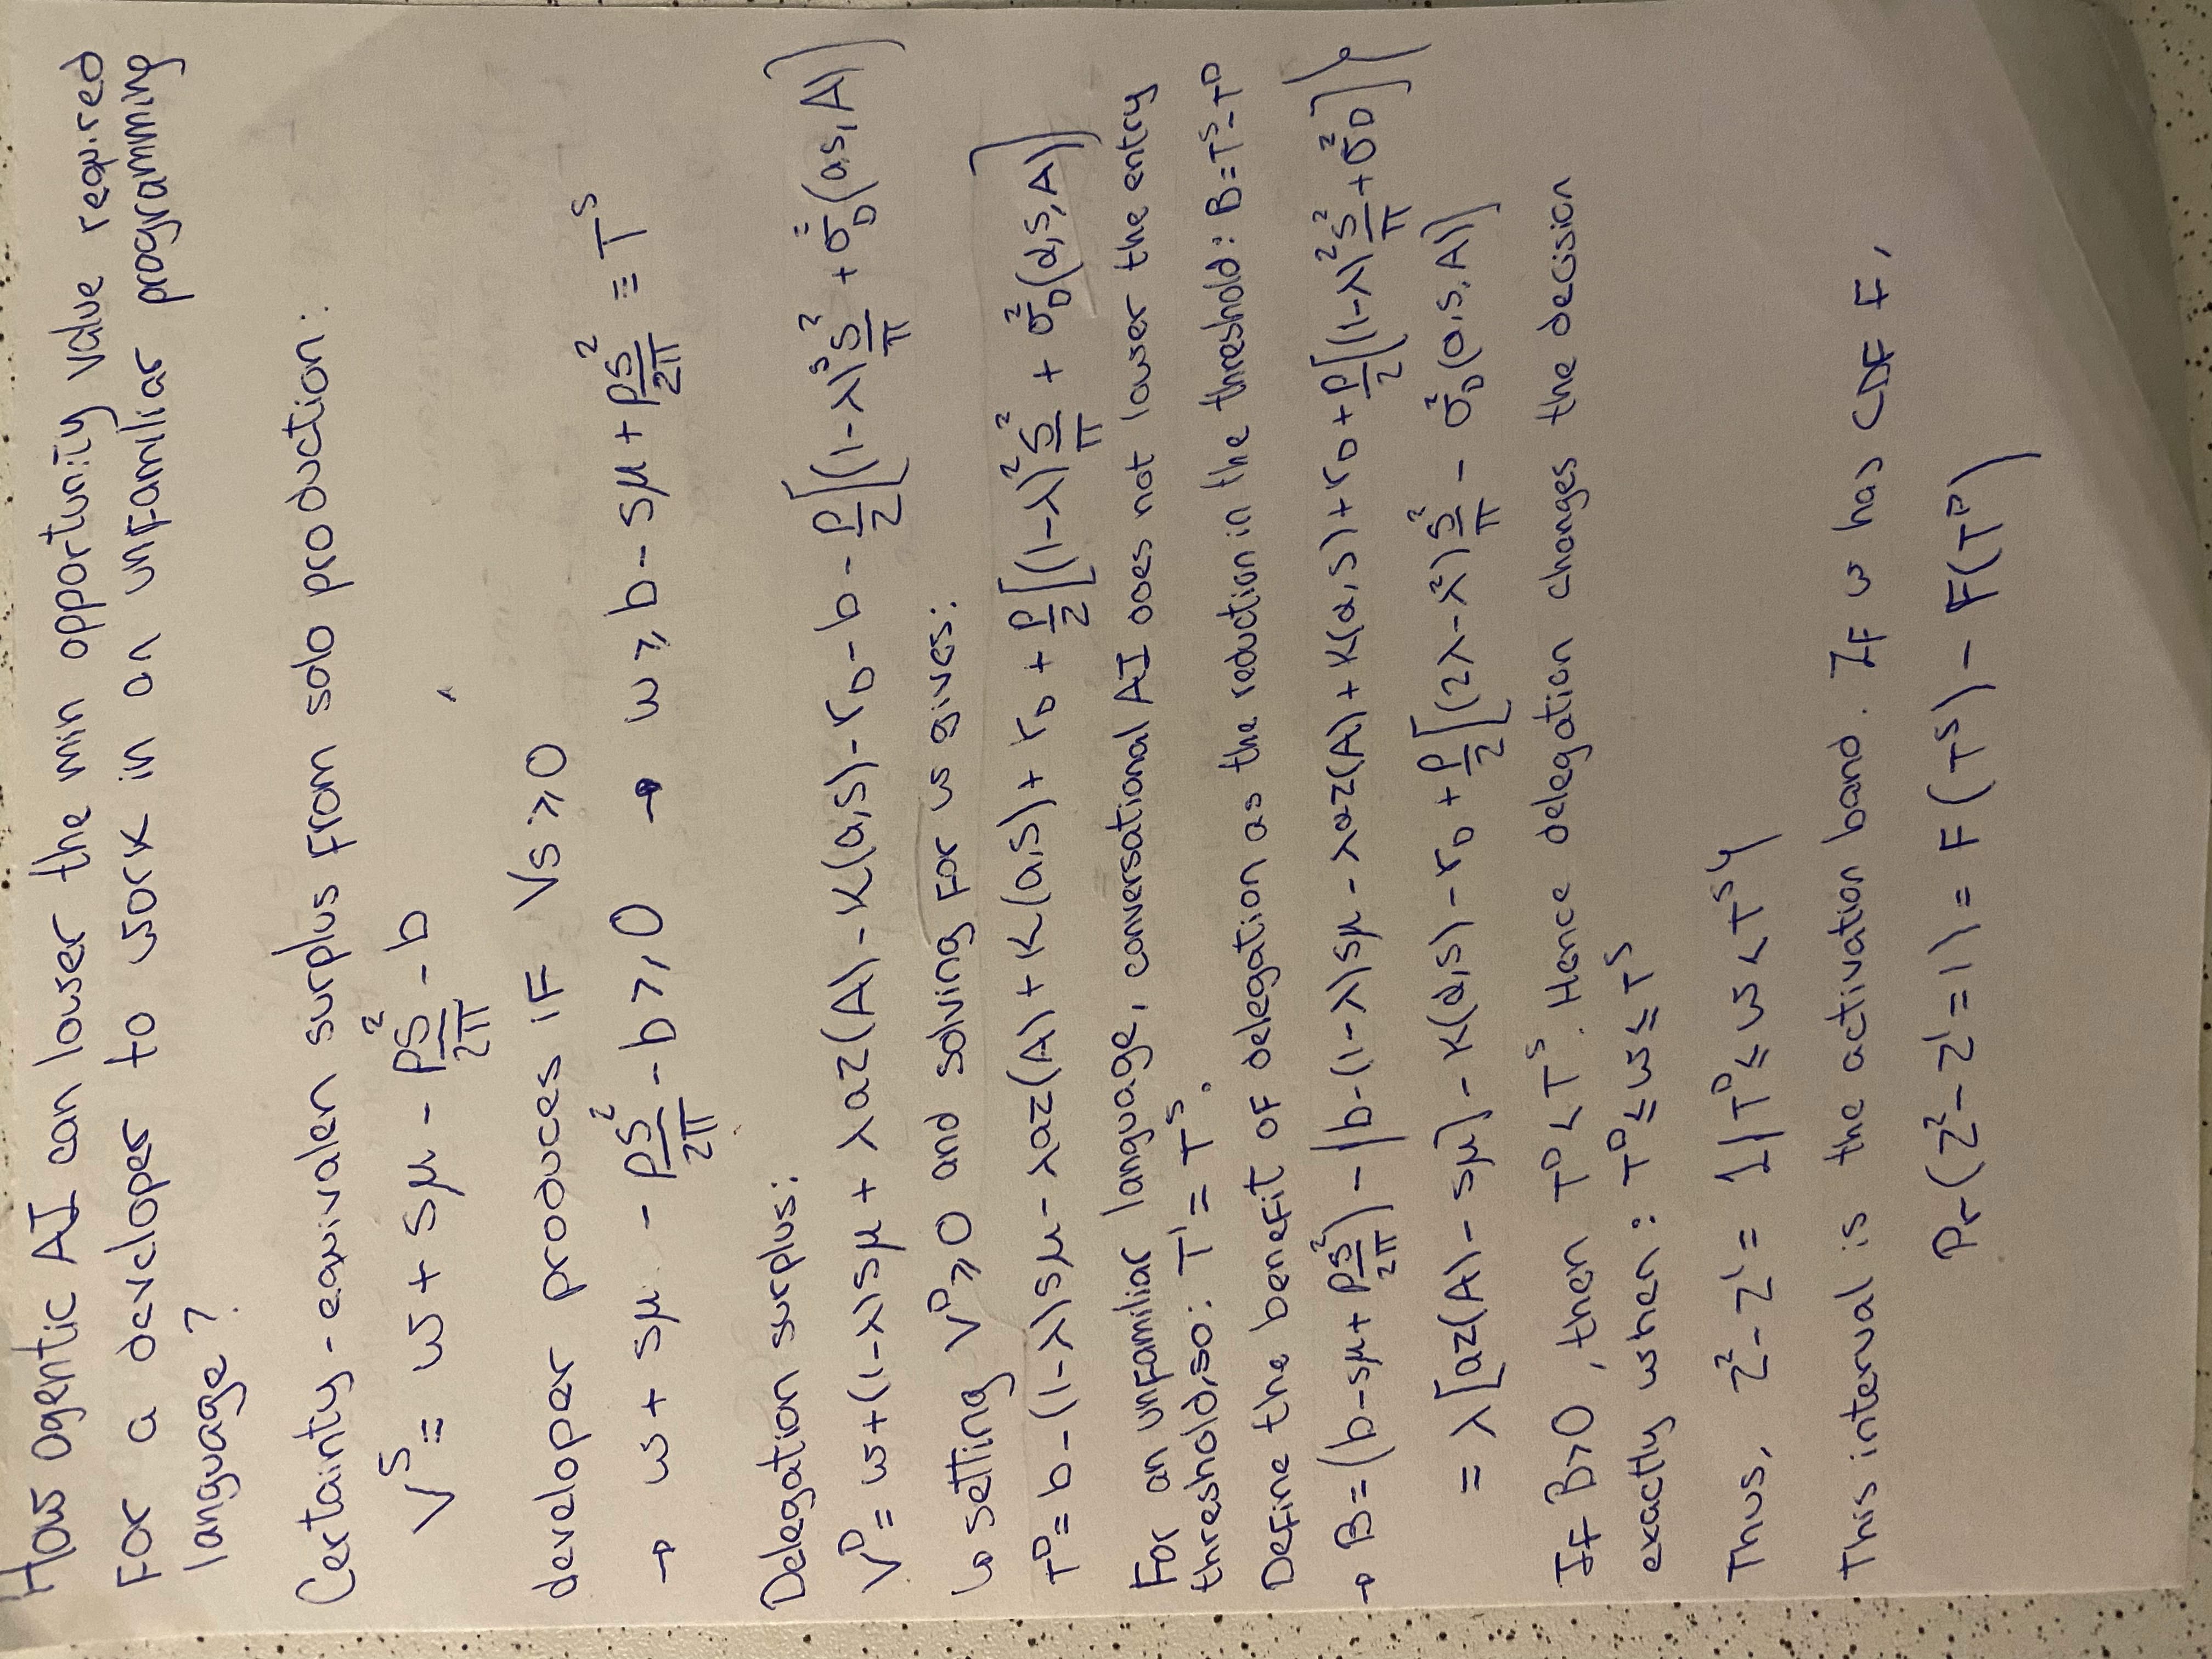
\includegraphics[width=.94\linewidth,height=6.30cm,keepaspectratio]{hand/selection-derivation.jpg}}
        \par\vspace{0.08cm}{\footnotesize\color{QXMuted}My handwritten selection derivation.\par}
      }{%
        \begin{beamercolorbox}[wd=.96\linewidth,ht=5.60cm,dp=.24cm,center]{qx placeholder}
          \vspace{1.64cm}
          {\Large\bfseries Handwritten photo goes here\par}
          \vspace{0.25cm}
          {\small Add \texttt{hand/selection-derivation.jpg}\par}
          \vspace{0.18cm}
          {\footnotesize Copy the four-line derivation in \texttt{hand/README.md}.\par}
        \end{beamercolorbox}
      }
    \end{column}
    \begin{column}{0.52\textwidth}
      \qxredblock{The AI claim I challenged}{%
        \small Flat pre-trends and outcome-side robustness make the portfolio
        expansion persuasive evidence for agentic delegation.
      }

      \vspace{0.08cm}
      \qxblueblock{What the derivation shows}{%
        \small
        With $\tau=0$,
        \[
          \widehat{\ATT}(0)=
          \beta\{\E[P\mid P\ge c]-\E[P\mid P<c]\}>0
        \]
        whenever $\beta>0$. The common project shock creates adoption and
        diversification together. Earlier pre-trends may still be flat because
        the shock arrives at $e=0$.
      }

      \vspace{0.08cm}
      \qxredblock{Verdict: \alert{mechanism-consistent, not mechanism-identified}}{%
        \small The paper documents a large, robust coincidence but cannot
        distinguish delegation from project selection. Causal identification
        needs exogenous adoption variation or a comparison with equally large
        non-agent productivity shocks.
      }
    \end{column}
  \end{columns}
\end{frame}

\end{document}
